\documentclass[12pt]{article}       %{amsart}

\usepackage[svgnames]{xcolor} 

\usepackage{amsmath, amsthm, ulem, graphicx, marvosym, fancyhdr, amscd, amssymb, float, enumerate}

%added as part of article format

\topmargin -.3in
\evensidemargin -.1in
\oddsidemargin -.1in
\textheight 8.5in
\textwidth 6.5in
\def\hs{\hspace{15pt}}

\newcommand*{\titleAT}{\begingroup % Create the command for including the title page in the document
\newlength{\drop} % Command for generating a specific amount of whitespace
\drop=0.1\textheight % Define the command as 10% of the total text height

\rule{\textwidth}{1pt}\par % Thick horizontal line
\vspace{2pt}\vspace{-\baselineskip} % Whitespace between lines
\rule{\textwidth}{0.4pt}\par % Thin horizontal line

\vspace{\drop} % Whitespace between the top lines and title
\centering % Center all text
\textcolor{Red}{ % Red font color
{\Huge Two-Dimensional Space Shooter Game with Roguelike Gameplay Mechanics}\\[0.5\baselineskip] % Title line 1
%{\Large with}\\[0.75\baselineskip] % Title line 2
{\Huge }} % Title line 3

\vspace{0.25\drop} % Whitespace between the title and short horizontal line
\rule{0.3\textwidth}{0.4pt}\par % Short horizontal line under the title
\vspace{\drop} % Whitespace between the thin horizontal line and the author name

{\Large \textsc{George Bateman BS CS \\* Jacob Cannon BS CS \\* Nicholas DeVoll BS CS \\* \vspace{3pt} Madison Silva BA CS}}\par % Author name

\vfill % Whitespace between the author name and publisher text

{\large \textsc{Faculty Mentor: Dr. Jorge Reyes Silveyra}}\par 

{\large \textsc{May 15th 2015}}\par

\vspace*{\drop} % Whitespace under the publisher text

\rule{\textwidth}{0.4pt}\par % Thin horizontal line
\vspace{2pt}\vspace{-\baselineskip} % Whitespace between lines
\rule{\textwidth}{1pt}\par % Thick horizontal line

\endgroup}

\setcounter{tocdepth}{2}

\begin{document}

\begin{titlepage}
\thispagestyle{empty}
\titleAT
\end{titlepage}

\newpage
\begin{titlepage}
\thispagestyle{empty}
\tableofcontents
\end{titlepage}

\begin{titlepage}
\thispagestyle{empty}
\listoffigures
\end{titlepage}

%\author{Madison Silva}\address{Pacific Lutheran University\\ Tacoma, WA 98447}%\email{silvamj@plu.edu}

\newpage

\section{Introduction}
\label{sec:intro}

\hs Video games have been a rapidly growing industry in the past 30 years \cite{History}. As such, there are a wide variety of genres and subgenres of games, each taking influence from and building upon successful games of the past. In some cases these games combine past elements in a way that create a new category of game. The goal of this project is to develop a game that will blend space-shooter elements from classic arcade games, such as Asteroids and Galaga, with randomized, challenging elements from more recent games such as The Binding of Isaac. These elements will include random usable items and equipment, permanent player death, and randomly generated level design. This combination will aim to provide players with new challenges that may not be available in current games. This game will be developed using Unity3D and will run in the Unity engine, which features robust tools that will allow us to manipulate nearly any element of the game quickly and with immediate feedback.

\section{Research Review}
\label{sec:Research}

\hs For the development of this project, we will develop a video game using Unity. The majority of the research time will be used to learn the functionality of Unity. Since Unity is a complete game engine and editor, the game creation process will not require the development of an engine. Other alternative engines, such as the graphics engine Ogre3D, would still require the implementation of a game engine in addition to creating the game \cite{Ogre}. Unreal Engine 4 was another considered engine, and included many features that would be useful to this project. However, many individuals have said that it is difficult for beginners to learn due to the lack of tutorials. Ultimately, we settled on Unity, since it has a wide range of tutorials to help us get started more quickly and will allow the majority of the project resources to go towards gameplay. development.

        Unity primarily uses $C\#$ as it’s scripting language. $C\#$ was created by Microsoft in 1997. It uses the .NET framework and is the most popular .NET language used today. It was influenced heavily by Java and C++, and it is intended to be friendly to the software development process so it has features such as uninitialized variable compatibility and automatic garbage collection \cite{Cadet}. Even though $C\#$ is a compiled language, Unity is still able to use $C\#$ code snippets as “scripts” because Unity is built in IDE (Monodevelop), compiles the code and packages it with game resources before runtime. This gives the games a robust set of tools, but allows the game to load and run quickly. \cite{Moles} 

	Our game strives to follow the principles set out by previous roguelike games. The term roguelike is a broad term used to describe video games that use random elements to create a replayable game that restarts the player on each subsequent playthrough. The original game that spawned this categorization was the game Rogue. Rogue was programmed at UC Santa Cruz in the 1980’s, using ASCII characters to take players on an adventure through a subterranean dungeon for the Amulet of Yendor. Once the game was released to others outside the developer, it spread rapidly throughout the college and the surrounding communities. Rogue inspired many other hits in the video game industry, including Diablo II, Faster Than Light, and The Binding of Isaac. \cite{Rogue}

	While developing non-player entities it is crucial to have an AI. Without an AI the entity becomes a stationary object and if they are an enemy that is not very exciting. One of the first step in creating a basic AI is choosing a pathfinding algorithm, so that the entity will move properly. An example of a basic but effective pathfinding algorithm is A*. Amit Patel defines A* as a combination of Dijkstra’s Algorithm and the Best-First-Search Algorithm \cite{A}. Dijkstra’s Algorithm searches all cells around the starting point moving out and searching the next farthest out cells in each direction until it finds the goal. In a game where time is valuable searching in the way would be inefficient. Best- First-Search(BFS) is faster because it searches only in the direction of the goal. This algorithm is not efficient for games because if there is an obstacle then the path that BFS takes can become inefficient. A* searches all vertices by favoring the ones in the direction of the goal, this helps it be more efficient like BFS but avoid obstacles more like Dijkstra’s. \cite{A}

	Finally, procedurally generated content will be used in order to build satisfying and challenging areas for the player. Procedural content generation is the process of designing an algorithm that can generate content at runtime. This fits in well with this project. With a relatively small number of inputs, the game can generate numerous different levels where the enemies encountered are found in different combinations. It also embodies the core idea of a roguelike game, changing the game every playthrough to challenge the player differently. There are a multitude of content generation algorithms, one of the common ones being Perlin noise, which actually refers to two algorithms created by Ken Perlin. These algorithms use a sum of different functions with varying amplitudes and frequencies in order to generate what is called a noise function. It is this function that is used to define different points of intensity. As it pertains to this project, these functions could be used to generate nebulae or star maps, giving a different visual experience to our player every time. \cite{PCG}

\section{Design}
\label{sec:Design}

\hs The following use cases and diagrams describe how the game will be implemented in the Unity game engine. While Unity is set up to handle the View portion and some of the Controller portion of the MVC architecture, we will have to supply part of the Controller and the Model portion in order to deliver our game.

\subsection{Use Case Scenarios} 
%%%
Scenario Name: {\bf PlayerDeath} \\
Participating Actor Instances:        \hspace{46pt} {\bf Player: PlayerEntity

					          \hspace{2.6 in}   Damager: DamageEntity 

					          \hspace{2.6in}    Heath: PlayerHP

						\hspace{2.6in}   Shield: PlayerShield} \vspace{10pt}  \\ 
Flow of Events: 
\begin{enumerate} 
\item {\bf Player }collides with {\bf DamageEntity}.
      \begin{enumerate}[a.]
       \item {\bf PlayerShield} decreases based on DamageEntity. 
       \item {\bf PlayerHP} decreases based on DamageEntity. 
                \begin{enumerate}[i.]
                 \item {\bf PlayerHP} is greater than zero, continue as normal.
                 \item{\bf PlayerHP} is less than or equal to zero, {\bf Player} dies.
                      \begin{enumerate}[1.]
                	\item {\bf Player} is deleted.
                	\item Explosion animation spawned in place of {\bf Player}.
		\item An end game menu prompts {\bf Player} to either play again or return to main menu.
		 \end{enumerate}
                \end{enumerate}
        \end{enumerate}
\end{enumerate}

%%%
\begin{center} \line(1,0){350} \end{center}
Scenario Name: {\bf LevelComplete} \\
Participating Actor Instances:        \hspace{46pt} {\bf Player: PlayerEntity

					          \hspace{2.6 in}   Boss: HostileEntity 

                                                      \hspace{2.6 in}   Rocket: Projectile 

					          \hspace{2.6in}    Item: InteractiveElement} \vspace{10pt}  \\ 
Flow of Events: 
\begin{enumerate} 
\item {\bf Boss} is destroyed by a {\bf Rocket} shot by the {\bf Player}.
\item {\bf Boss} will enter an animation where it explodes and drops an {\bf Item}.
\item {\bf Player} has a grace period where they can pick up the {\bf Item} dropped by the boss, and then they’re transported to the shop and inventory management menus.
\item After they are done with the end of level menus, {\bf Player} is taken to the beginning field of play for the next level. 
\end{enumerate}

%%%
\begin{center} \line(1,0){350} \end{center}
Scenario Name: {\bf LeavingFieldOfPlay} \\
Participating Actor Instances:        \hspace{46pt} {\bf Player: PlayerEntity

					          \hspace{2.6 in}  Projectile: PlayerKiller}  \vspace{10pt}  \\ 
Flow of Events: 
\begin{enumerate} 
\item {\bf Player} leaves the field of play.
\item Warning alarm sounds, warning flashes on screen.
      \begin{enumerate}[a.]
       \item {\bf Player} chooses to turn around and return to field of play, everything returned to normal.
       \item {\bf Player} advances farther out of the field of play.
                \begin{enumerate}[i.]
                \item {\bf PlayerKiller} kills {\bf Player}.
	     \item PlayerDeath().
                \end{enumerate}
        \end{enumerate}
\end{enumerate}

%%%
\begin{center} \line(1,0){350} \end{center}
Scenario Name: {\bf GenerateLevel} \\
Participating Actor Instances:        \hspace{46pt} {\bf LG: LevelGenerator

					          \hspace{2.6 in}   GM: GameManager}  \vspace{10pt}  \\ 
Flow of Events: 
\begin{enumerate} 
\item {\bf GM} notifies {\bf LG} that a level needs to be generated.
\item {\bf LG} creates a level layout.
      \begin{enumerate}[a.]
      \item If {\bf LG} determines that the level layout is navigable and correctly generated
                \begin{enumerate}[i.]
                \item The level is generated
                \end{enumerate}
      \item If {\bf LG} determines the the level layout is not navigable and is incorrectly generated
                \begin{enumerate}[i.]
                \item The {\bf LG} creates another layout and checks again.
                \end{enumerate}
        \end{enumerate}
\end{enumerate}

%%%
\begin{center} \line(1,0){350} \end{center}
Scenario Name: {\bf MoveAndShoot} \\
Participating Actor Instances:        \hspace{46pt} {\bf Player: PlayerEntity

					          \hspace{2.6 in}   Bullet:Projectile}  \vspace{10pt}  \\ 
Flow of Events: 
\begin{enumerate} 
\item {\bf Player} presses a movement button, which defaults to the WASD keys, while simultaneously pressing a fire button, which default to the $ \uparrow \downarrow \leftarrow \to $ arrow keys.
\item {\bf Player} moves in the direction of the movement button pressed, while {\bf Bullet} is fired in the direction of the fire button pressed.
\item {\bf Player} continues moving in the way of the first directional input until an additional input is received, at which time {\bf Player} will begin to move in the way of the second directional input. {\bf Bullet} travels in the direction it was initially shot without the possibility of changing direction.
      \begin{enumerate}[a.]
      \item The {\bf Bullet} travels until it collides with another entity.
                \begin{enumerate}[i.]
                \item The {\bf Bullet} causes damage to that entity and terminates itself.
                \end{enumerate}
      \item The {\bf Bullet} travels until it fizzles out of the view of {\bf Player}.
                \begin{enumerate}[i.]
                \item The {\bf Bullet} terminates itself.
                \end{enumerate}
        \end{enumerate}
\end{enumerate}

%%%
\begin{center} \line(1,0){350} \end{center}
Scenario Name: {\bf BulletFizzle} \\
Participating Actor Instances:        \hspace{46pt} {\bf Player: PlayerEntity

					          \hspace{2.6 in}   Bullet:Projectile}  \vspace{10pt}  \\ 
Flow of Events: 
\begin{enumerate} 
\item {\bf Player} shoots a {\bf Bullet}.
\item {\bf Bullet} does not hit anything within the view of the {\bf Player}.
\item {\bf Bullet} travels out of the view of the {\bf Player}.
      \begin{enumerate}[a.]
       \item The {\bf Bullet} collides with an entity
                \begin{enumerate}[i.]
                \item The {\bf Bullet} causes damage to that entity, and terminates itself.
                \end{enumerate}
      \item The {\bf Bullet} does not collide with anything.
                \begin{enumerate}[i.]
                \item The {\bf Bullet} is terminated after a short distance.
                \end{enumerate}
        \end{enumerate}
\end{enumerate}

%%%
\begin{center} \line(1,0){350} \end{center}
Scenario Name: {\bf PauseGame} \\
Participating Actor Instances:        \hspace{46pt} {\bf Player: PlayerEntity }  \vspace{10pt}  \\ 
Flow of Events: 
\begin{enumerate} 
\item {\bf Player} presses the pause button.
\item A menu pops up with three options; resume game, options, and exit game.
      \begin{enumerate}[a.]
      \item If resume game is chosen, the menu exits and gameplay is resumed.
      \item If options is chosen, the game state is maintained and the {\bf Player} is taken to the options menu.
      \item If exit game is chosen, a sub menu pops up giving three options; exit to menu, exit game, return to menu.
                \begin{enumerate}[i.]
                \item If exit to menu is chosen, {\bf Player} is taken to the main screen view.
                \item If exit game is chosen, the game is closed.
                \item If return to menu is chosen, the {\bf Player} is navigated back to the prior menu.
                \end{enumerate}
        \end{enumerate}
\end{enumerate}


\subsection{Use Case Model}
Figure \ref{Use Case Model} shows which external actors participate in each of the Use Case Scenarios included.

\begin{figure} [H]
\centering
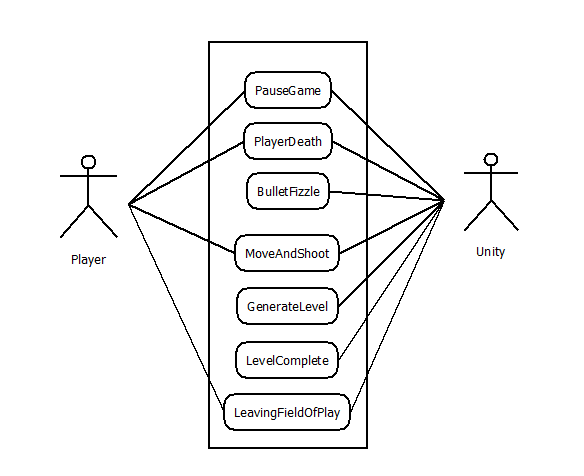
\includegraphics[width=5.5in]{UseCaseModel1.png}
\caption{Use Case Model} \label{Use Case Model}
\end{figure}

\newpage
\subsection{Sequence Diagram}
The sequence diagram represented in Figure \ref{PlayerDeath}  corresponds to the use case PlayerDeath, and outline the process behind the player being hit with a projectile to a death state, followed by the appropriate response by the {\it GameController}. The branching paths occur if the Projectile killed the player or if they had an item that could revive them. Sequence diagrams for other use cases are functionally similar, albeit with a few differing actors and method calls.
\begin{figure} [H]
\centering
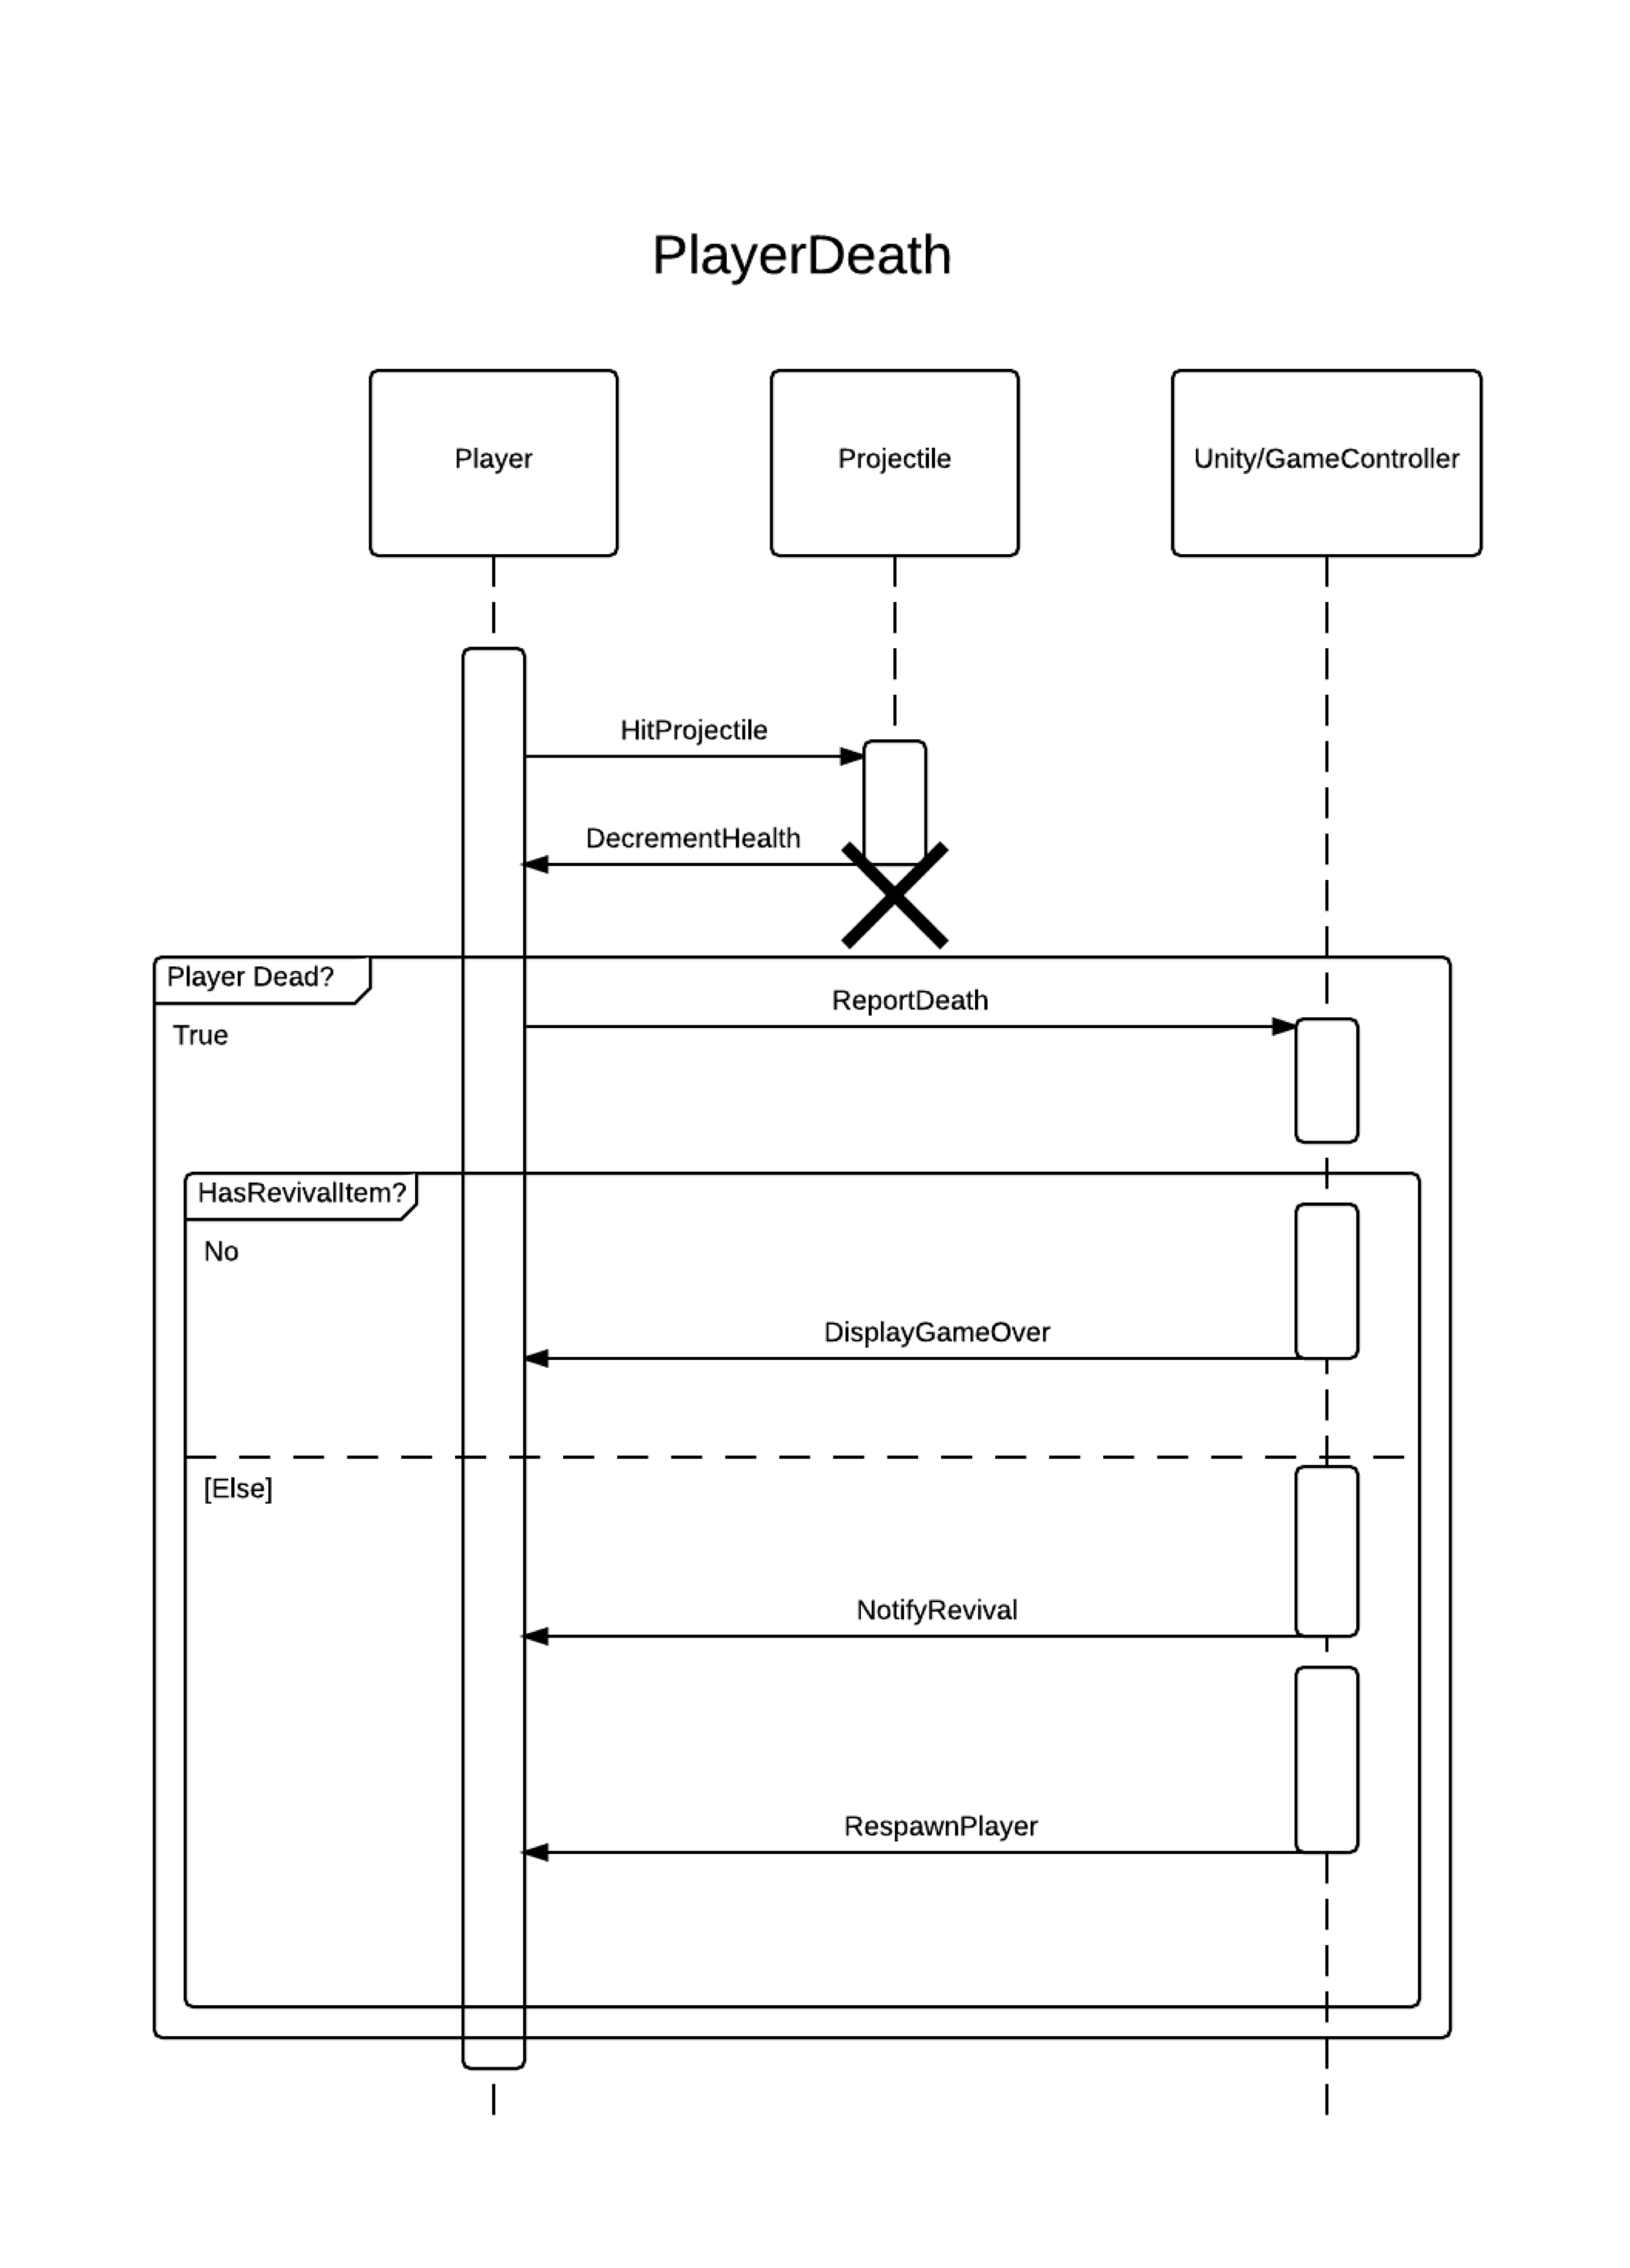
\includegraphics[width=4.75in]{PlayerDeath.png}
\caption{Player Death Sequence Diagram} \label{PlayerDeath}
\end{figure}

\subsection{UML Diagram}
\hs In Figure \ref{UML} shows the core class design for the game and the relations that classes will have with each other. Classes will be interacting with existing classes of the Unity engine. {\it GameManager} will be a singleton class that will be responsible for holding the {\it Player Entity}, this way the game can easily transport the {\it Player} between scenes without risk of creating a duplicate {\it Player}. {\it GameController} will handle everything that happens inside the level itself, and will be able to do this with the onAwake() function, provided by Unity, that activates when the script has been loaded into the scene. The {\it Entity} object will provide a basis of all entities in-game that will be able to move and react to the game state, including the {\it Player}. The {\it Ship} class will be a prefab handled by Unity that will allow us to instantiate an {\it Entity} object with certain variables from the start. Our {\it Item} and {\it Weapon} interfaces will handle items and weapons picked up in the game, respectively. It is important that there is a distinction between the two, as all {\it Weapons} are {\it Items} but not all {\it Items} are {\it Weapons}.

\begin{figure} [H]
\centering
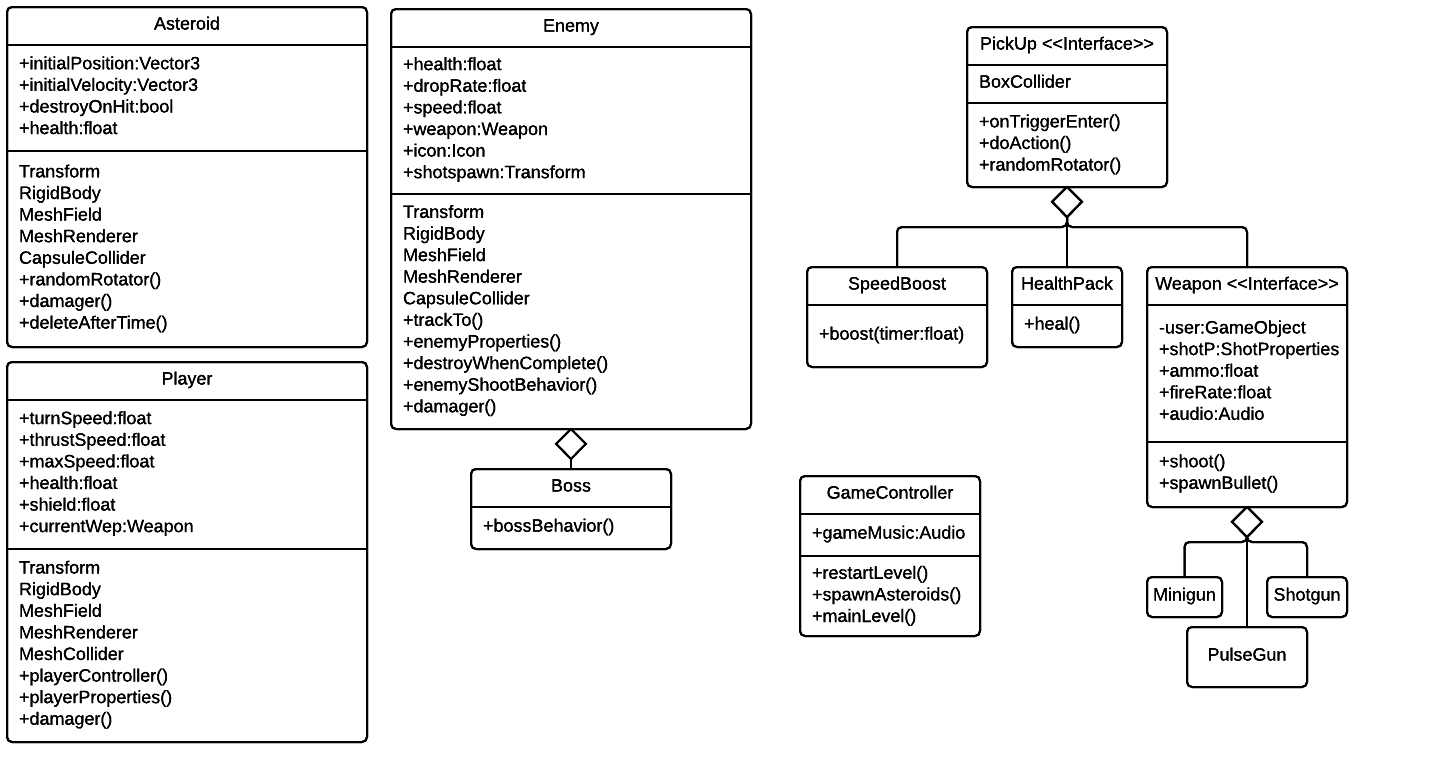
\includegraphics[width=7.3in]{FinalUMLHorizontal.png}
\caption{UML Diagram} \label{UML}
\end{figure}

\subsection{State Diagram}
Figure \ref{StateDia} describes the transitions between various scenes and menus in the game. Each state corresponds to either a Unity scene or a GUI child menu.

\begin{figure} [H]
\centering
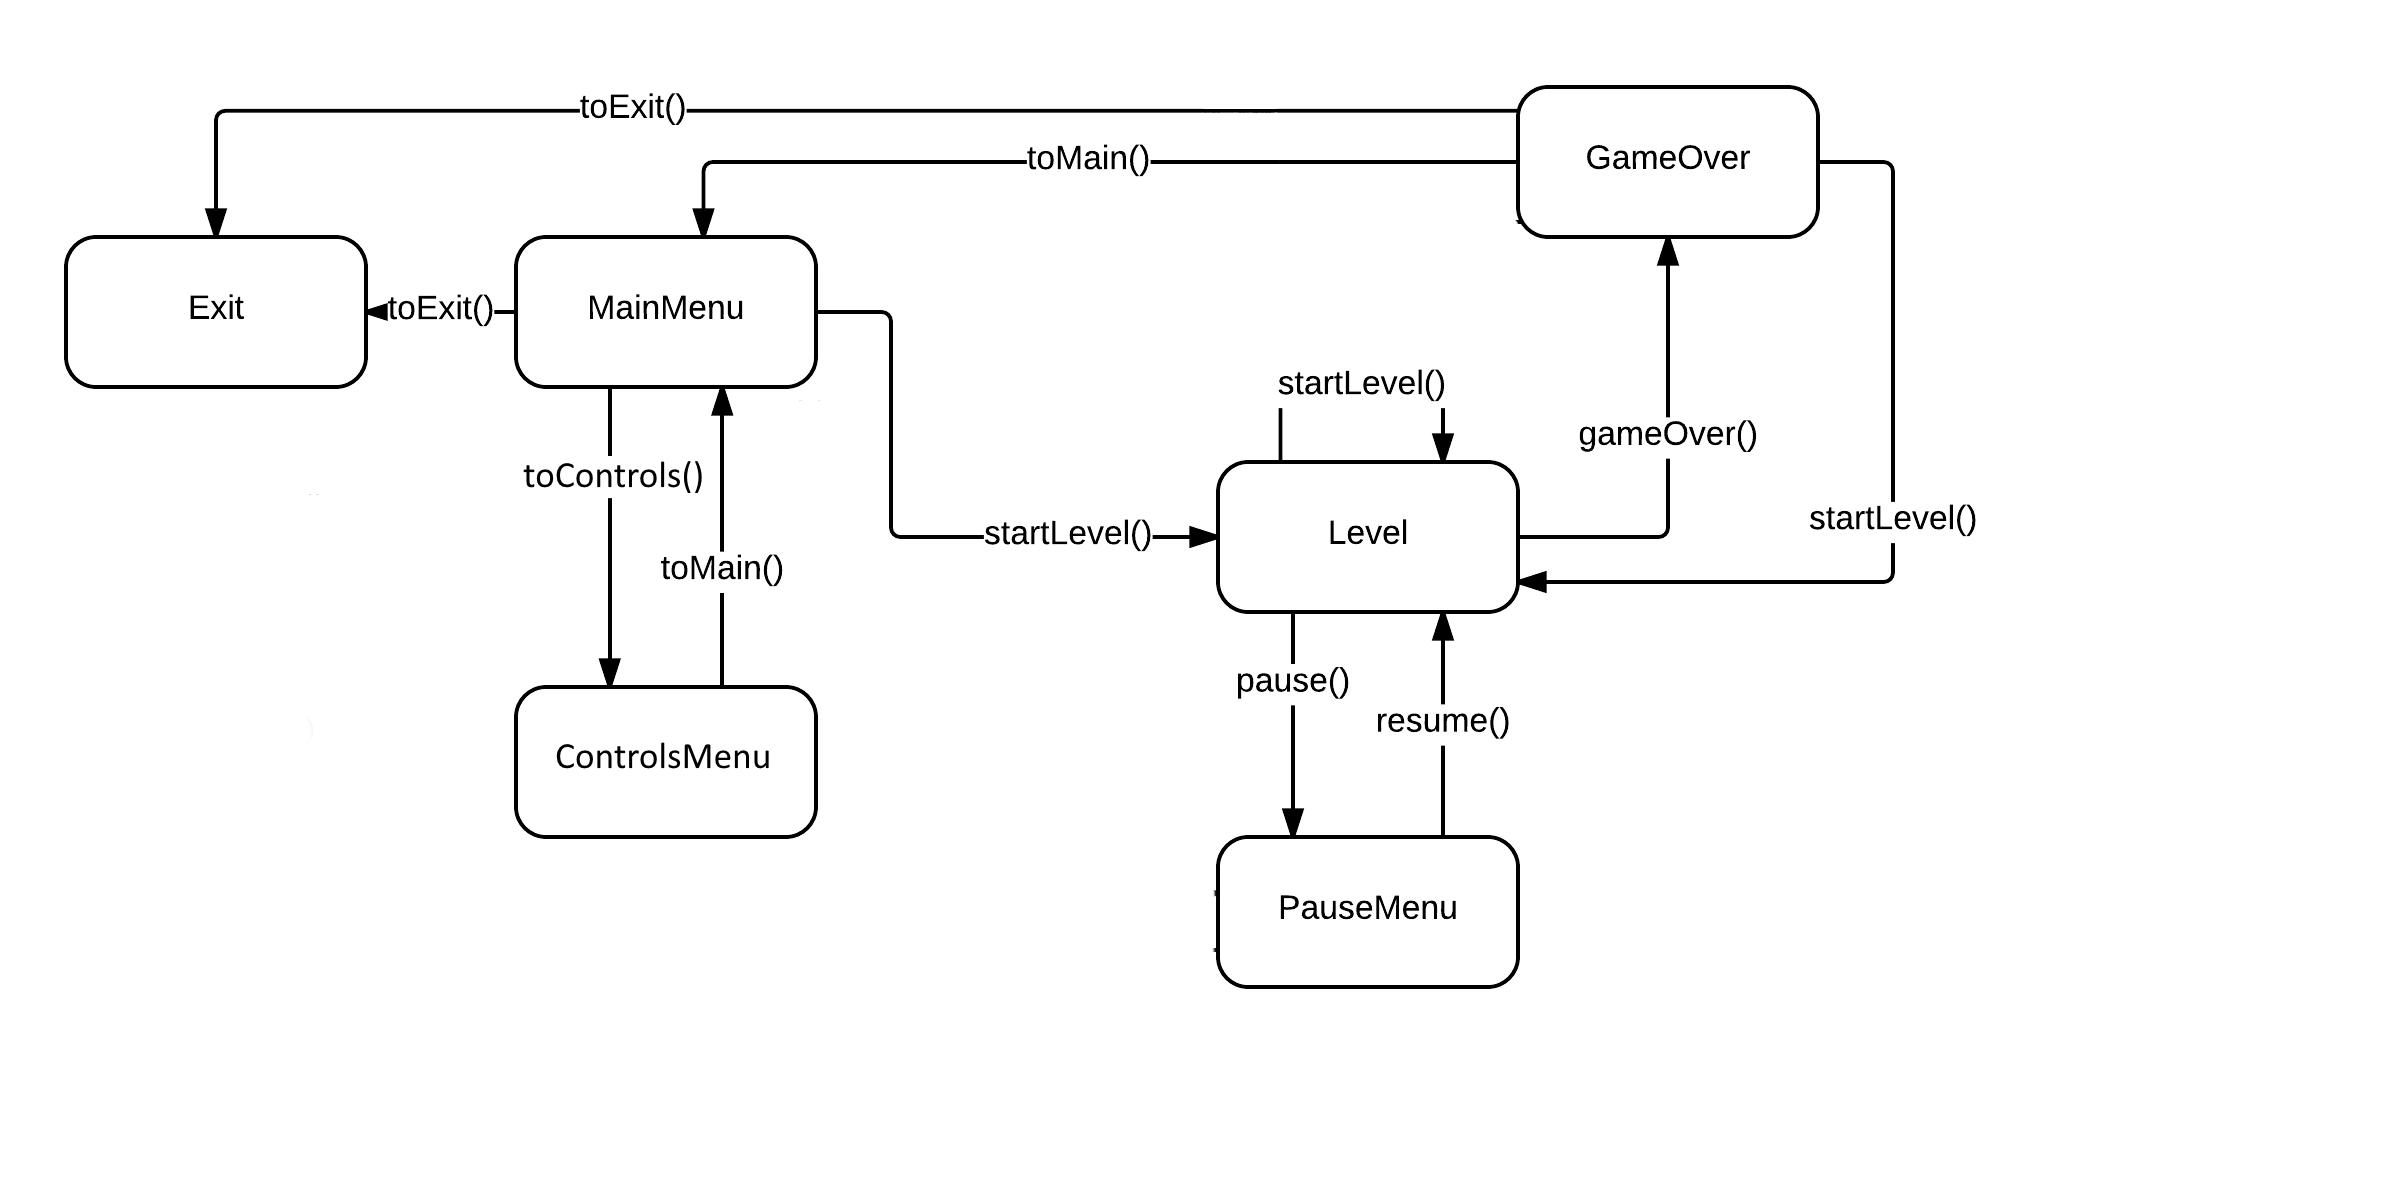
\includegraphics[width=7in]{PewPewStateDiagramFinal.png}
\caption{State Diagram} \label{StateDia}
\end{figure}

\section{Gameplay Design}
\label{sec:GPdesign}

Games are dynamic pieces of software that focus on delivering exciting or interesting experiences to players, gameplay design is as important as backend design. What follows is the basic design for the aspects of the gameplay that the player will see.

\begin{itemize}
\item Player controls: The player controls a small spaceship, and navigates through a space environment. As seen in Figure \ref{Controls}, the player will move with the WASD keys; pressing a key will cause the ship to accelerate in that direction. Acceleration speed will not be instantaneous and the player will not stop automatically, in order to simulate a sense of weight and the lack of friction in space. Shooting will be controlled by the arrow keys on the keyboard. Pressing an arrow key will cause shots to be fired in that direction. Since movement and shooting are separate, the player may move in one direction and fire in another. Usable items can be activated by pressing the spacebar. The controls are intended to transfer over to a controller relatively easily, so the player may control moving and shooting with the left and right analog stick respectively. The controls diagram is located at section 4.1 of this document.

\item Player’s ship: The players ship will have it’s own health and shield values. The shield will be a rechargeable defense that will be able to absorb a number of shots before the players ship takes permanent health damage. Recharging of the shield will occur over time. The ship’s health is the amount of damage the ship can sustain before it explodes and the player loses. It will not regenerate automatically like the shield, but items will be able to restore it.

\item Pick-ups:  The ship will also be able to pick up passive items that will change firing traits or speed.{\textcolor{Red}{[CHANGE]}}

\item Radar: 

\item Standard Shooting:

\item Predictive Shooting: 

\item Enemies: The main goal of enemy ships is to kill the player ship. There are two main strategies the enemies will utilize to accomplish this. Certain enemies will shoot at the player, forcing the player to dodge if they want to survive, while other enemies will attempt to ram the player to deal damage. As such, there are enemy ships that will fly around in basic patterns while shooting at the player, and there are enemy ships that will charge straight at the player to prevent them from staying still for too long. Additionally, there will be “enemy” obstacles such as asteroids that will fly on screen to force players to be aware of their surroundings. These obstacles have no set objective and can hit enemy ships as well.

\item Level design: Enemy placement will play a critical role in the design of levels. The placement of enemies needs to be dense enough so that there is a challenge but  sparce enough so that every level is possible and does not feel the same. Since the game takes place in space, there will not be traditional level elements such as walls and floors. However, there may need to be other obstacles that guide the player‘s movements such as debris or very large ships.

\item Weapons: Weapons will need to serve two functions: give the player a variety of gameplay options and motivate the player to explore a different gameplay style. For instance, a laser may allow the player to shoot a long range beam that pierces enemies but does not deal much damage, while a shotgun may reward the player with a more damaging weapon, but require the player to engage with enemy ships from a much closer range. The player will be able to switch out weapons such as these to better fit their playstyle.

\item Items: The majority of the items in the game will provide a general bonus to the player without requiring additional action from the player. These could include upgrades like increased shield or hull capacity, increased damage, or faster ship acceleration. Additionally, there will be various items that the player can activate by pressing the Activate Item key that will provide the player with some benefit when used. For instance, a time bomb may temporarily slow down enemy ships and projectiles to allow the player to dodge them more easily.

\item Bosses: Bosses will give the player a final challenge before ultimately reaching the end of the game and winning. Bosses will shoot large amounts of projectiles to making dodging difficult for the player. Additionally, the boss will have a predictive shooting projectile to increase the difficulty further. Finally, bosses will have a larger amount of health than the average enemy. Defeating a boss will end the game and display a win screen.

\item Story - The Player is an explorer trying to reach the other side of the Universe to meet aliens that sent a treasure map to earth. The Player keeps in close contact with General Weathersbee who guides them to the last known location of the aliens. 

\item Art/models: The assets and models used in this project will all be free from the Unity store. We will use our own creativity to make all of the assets blend together in a cohesive way. We are using a black with star background for the main level, and then varying space themed backgrounds for the other scenes. The font Huxely is through out the game to tie the art all together.  

\item Music/ sound: Sound effects and music will be retrived from the Unity store and other creative commons sites. It will attempt to replicate a space environment similar to other space themed games. For example the laser gun will have a "pew pew pew" sound. 

\end{itemize}

\subsection{Controls Diagram}

\begin{figure} [H]
\centering
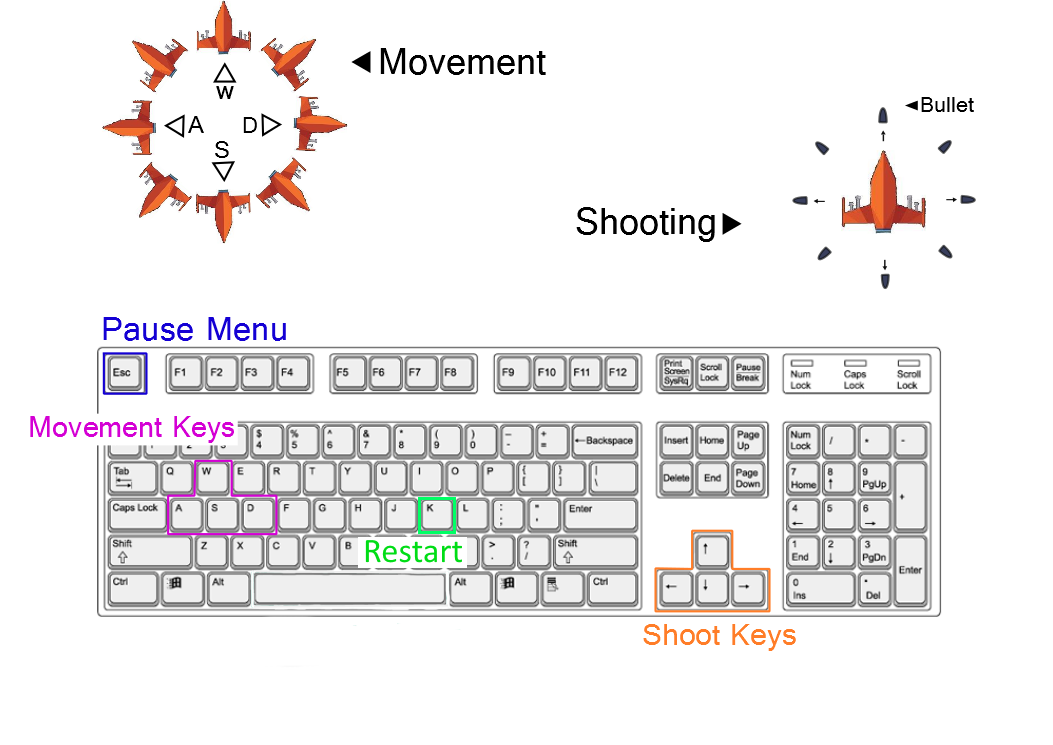
\includegraphics[width=6.3 in]{ControlDiagramFinal.png}
\caption{Controls Diagram} \label{Controls}
\end{figure}

\subsection{Miscellaneous}
\hs {\bf Testing plans}: The group members will play the game every step of the way to make sure that the individual additions to the project are functioning as expected. Once there is a version of the game that allows a player to navigate an environment and fight basic enemies, the group will reach out others to play it and give feedback in the form of a simple survey. 

{\bf Victory conditions}: The player will achieve victory by completing each area that is generated without dying. The game is planned to culminate with a boss fight, and defeating this boss will trigger victory and end the game.

{\bf First Minute}: The player enters the game with their chosen ship, and can immediately start exploring the area in which they spawn. They will see the controls of the game described on the field, introducing new players to the game. After discovering how to control their ship, players will be able to leave the starting area in a single direction, leading them to the first area of the game. In this first area, enemies will be created at the other side of the field. The player must defeat these enemies to clear the field and move on. As the player moves about the field, the enemies start reacting, moving towards the player to defeat him. When battle resolves, any dropped items and currency are picked up by the player, and they are given a choice where to go next.

\section{History of Work}
\label{sec:history}
This section describes the completed work, current status, and future plans that are to be included to the project.

\subsection{Work Completed}

\hs The Unity website offers in-depth tutorials on how to create basic games using the Unity engine. We have completed two specific tutorials in preparation for this project: The “Beginner” rated project, entitled “Space Shooter”, and the “Intermediate” rated project, “Project: Stealth”.

  The “Space Shooter” tutorial introduced us to the basics of Unity, and explained how to use the engine to create a top-down, two-dimensional space shooter game using given assets, including a three-dimensional ship model, a provided background, and models for asteroids and enemy ships. It also provided sample scripts to use for the completed game, written in $C\#$. The completed project spawned varying waves of asteroids that the player would have to either shoot or dodge, with a score counter incrementing every time the player shot an asteroid and the game ending when the player took damage from colliding with an asteroid and dying.

 The “Project: Stealth” tutorial went into much more depth than the “Space Shooter” tutorial, and guided us through making a fully functional three dimensional stealth-based game. Using provided assets, the tutorial showed us how to use animations to change collisions, enemy AI that reacted to various events that the player had some limited control over, and advanced $C\#$ scripting work that went into more detail than the basics in the “Space Shooter” tutorial. The finished project was a fully functional game in which the player would attempt to reach the end of a level without alerting various AI guards.

  We intend to use many of the elements presented in both of these tutorials as building blocks in our own game. From the “Space Shooter” tutorial we intend to use the fundamental concepts presented in the tutorial, namely scripting, collisions, and two-dimensional top-down shooter action, in our product. From the “Project: Stealth” tutorial we intend to use some of the overall concepts, such as enemy artificial intelligence and events occurring in response to our game state in our product.

\subsection{Current Status}

Development is starting to move out of preliminary stages as we get the group back together for spring semester. We have finished mutiple Unity tutorials and have a basic foundation of the game. We are currently working on creating a new time table to get develpment on track. The design document was completed and turned in on December 18th, 2014, and an updated version of the document was turned in February 19th, 2015. 

\subsection{Future Work}
The following are tasks that still need to be completed in order to produce a functional polished game.

\begin{enumerate}[A.]
{\bf \item Research and Design Tasks:}
     \begin{enumerate}[a.]
	\item Game Design
        \begin{enumerate}[i.]
	\item Story- Come up with a complete story that includes a purpose and a goal. This will enhance the gameplay and get people interested in playing the game.
         \item Art - Pick what art style the game will follow. Start gathering backgrounds  
        \item Models
	\end{enumerate}
        \item Pathfinding Unity Tutorial - Find and complete a tutorial on Unity that focuses on the pathfinding aspects of the A.I.
	\end{enumerate}

{\bf \item Implementation Tasks:}
\begin{enumerate}[a.]
	
\item Entity movement - The player and AI will have the ability to control in game entities to affect gameplay. 

\item Collisions - The game will detect collisions between different entities, affecting movement and gameplay.

\item Artificial Intelligence

\begin{enumerate}[i.]
\item Enemy response - The enemy AI will respond to player actions, influencing their own..
\item Follower movements - Follower ships will follow the player around and shoot at enemies as they approach.
\item Enemy spawning - A system that is dedicated to the spawning of enemies and obstacles upon loading a level.
\end{enumerate}

\item Inventory Control System
\begin{enumerate}[i.]
\item Sorting- Player will be able to move items around in their inventory.
\item Equipping - Player will be able to equip a set amount of items into a number of different equipment slots. Equipping items will give the player a number of different benefits.
\item Selling- Player can sell extra or unwanted items at a shop to clean out their inventory.
\end{enumerate}

\item User Interface
\begin{enumerate}[i.]
\item Heads up display- The information elements that will display vital information during gameplay.
\item Minimap- A small map that shows the location of enemies and objectives relative to the player.
\item Shop window- An interactive window that displays items available for purchase.
\end{enumerate}

\item Audio
\begin{enumerate}[i.]
\item Sound Effects - Actions that the player can take, as well as certain environmental effects, will have sounds associated with them.
\item Music - Different soundtracks will play in the background of differing areas and menus.
\end{enumerate}

\item Lighting - Lighting systems will add dynamic lighting and ambience to make key entities more visible.

\item Randomly generated levels - Levels will be generated upon loading each one differing from other level generations.

\item Multiple artificially controlled enemies
\begin{enumerate}[i.]
\item Boss Enemies - An enemy that provide both a significant challenge and an extra reward.
\item Unique Enemies - differing types of enemy entities
\end{enumerate}

\item Graphical Effects
\begin{enumerate}[i.]
\item Animations - animations will be used to create a smooth, interesting visual experience.
\item Particle Effects - particle effects will be included to enhance certain actions, i.e. thrusters.
\item Parallax Backgrounds
\end{enumerate}

\item Interactive background elements - Some background elements will interact with the player. For instance, a planet in the background might bombar the player with explosive armaments.

\end{enumerate}
\end{enumerate}

\section{Timetable}
\label{sec:time}
Figure \ref{Time} describes the planned development cycles for creating the game.

\begin{figure} [H]
\centering
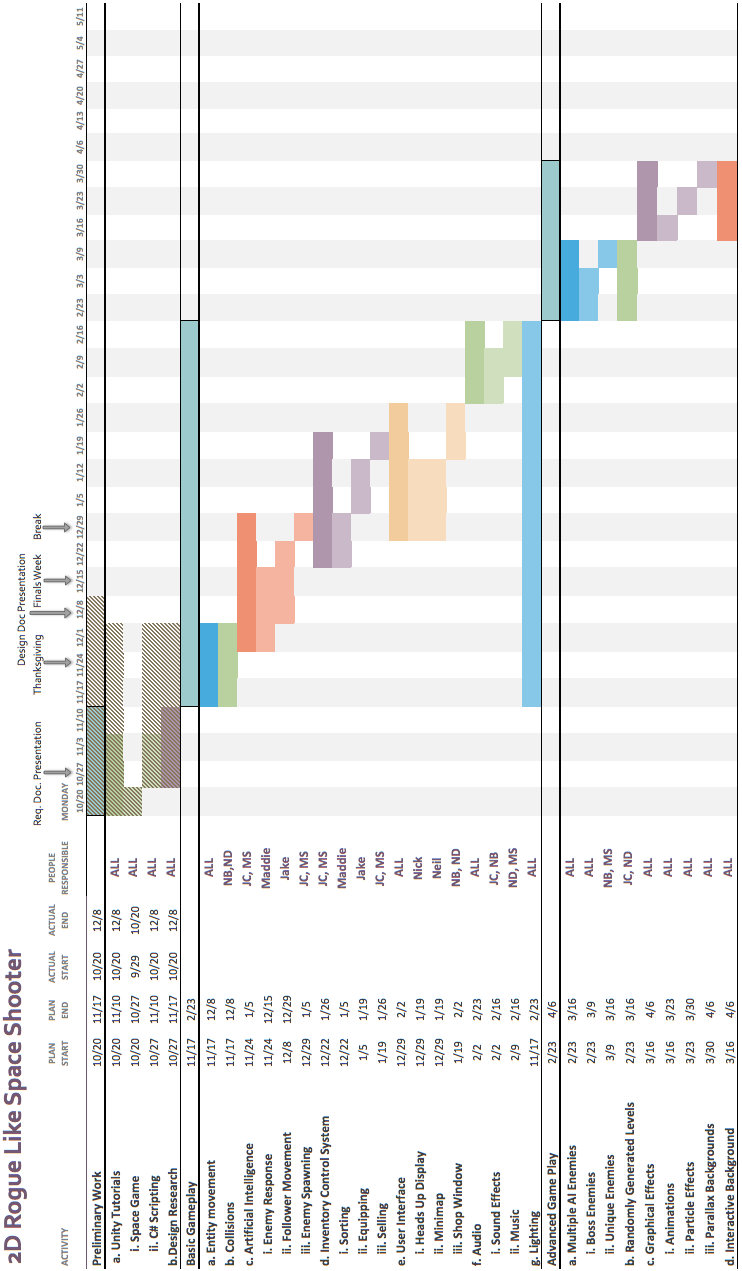
\includegraphics[width=4.3 in]{TimeTableDec.png}
\caption{Current Time Table} \label{Time}
\end{figure}


\newpage
%\section{References}
%\label{sec:ref}

\begin{thebibliography}{99}

\bibitem{History} Ringo, D. History of Gaming: A Look at How It All Began. Public Brodcasting Service, n.d. Retrieved October 20, 2014, from PBS: http://www.pbs.org/kcts/videogamerevolution/history. 

\bibitem{Tutorials} Tutorials. Unity Technologies, n.d. Retrieved October 15, 2014, from Unity: http://unity3d.com/learn/tutorials/modules.

\bibitem{C} Creighton, R. Unity 4.x Game Development by Example Beginner's Guide, 3rd ed. Packt Publishing, Birmingham, UK, 2013.

\bibitem{Edgar} Edgar, T. Latex-slides. Department of Mathematics Pacific Lutheran University, Tacoma, WA, September 2011. PDF. 

\bibitem{Rogue} A Brief History of Roguelikes, Kill Screen Daily. Retrieved November 14, 2014 from Kill Screen Daily, INC: http://killscreendaily.com/articles/brief-history-roguelike/.

\bibitem{PCG} Procedural Content Generation Wiki. Retrieved December 4, 2014 from: http://pcg.wikidot.com/.

\bibitem{Cadet} Cadet, H. A Brief History of C Sharp.  N.p., n.d. Retrieved November 13, 2014 from Hernando Cadet Technology:  http://www.hernandocadett.com/content/brief-history-c-sharp/.

\bibitem{E} Elias, H. Perlin Noise. Retrieved December 6, 2014 from: http://freespace.virgin.net/hugo.elias/models/m\_perlin.htm.

\bibitem{Moles} Moles, S. How Does Unity Use $C\#$ as a Scripting Language? N.p., n.d. Retrived: November 13, 2014 from Game Development Stack Exchange: http://gamedev.stackexchange.com/questions/51350/how-does-unity-use-c-as-a-scripting-language.

\bibitem{Ogre} About Object-Oriented Graphics Rendering Engine. Retrived November 2014 from Torus Knot Software: http://www.ogre3d.org/about/

\bibitem{Guide} Stevens, P. and Tenzer J. GUIDE: Games with UML for Interactive Design Exploration. 
{ \it Laboratory for Foundations of Computer Science School of Informatics}. Retrived November 16, 2014 from University of Edinburgh: http://homepages.inf.ed.ac.uk/perdita/guide.pdf.

\bibitem{UML} UML for games. November 2003. Retrived November 16, 2014 from GameDev.Net LLC: http://www.gamedev.net/topic/192120-uml-for-games/

\bibitem{A} Patel, A. Introduction to A*. Red Blob Games, 1997. Retrived November 18, 2014 from Stanford University: http://theory.stanford.edu/~amitp/GameProgramming.
 
\bibitem{GDD} Effectively Organize Your Game's Development With a Game Design Document. Tutsplus. Gamux. Envato, November 11, 2011. Retrived November 18, 2014 from Tutsplus: http://code.tutsplus.com/articles/effectively-organize-your-games-development-with-a-game-design-document--active-10140. 


\end{thebibliography}

\newpage

\section{Glossary}
\label{sec:gloss}

{\bf{AI}} - Artificial Intelligence, in our case directing the actions of the NPCs. \\
{\bf Boss} - A unique hostile entity that appears at the end of a level. \\
{\bf Entity} - An object that can interact with other objects in the game. \\
{\bf Field of Play} - The area in which a player will interact with obstacles, enemies, and other events. \\
{\bf HP} - Health points, a measure of the players health level often represented as either a fraction or bar. \\
{\bf Level} - A collection of similarly challenging fields of play culminating in a boss. \\
{\bf NPC} - Non Player Characters, e.g., any enemies or passive characters that act in the game that are not controlled by the player. \\
{\bf Parallax} - The effect whereby the position or direction of an object appears to differ when viewed from different positions, e.g., elements far from the camera appear to move more slowly than foreground elements. \\
{\bf Prefab} - A function supported by Unity that allows for predefined object specification and quick entity instantiation. \\
{\bf Ramming} - When one entity attacks another through direct collision. \\
{\bf Roguelike Game} - A game that is distinct because of two important characteristics:
Has highly randomized gameplay with a large amount of replayability. 
Permanent death, meaning if the main protagonist dies, the game ends and the player must restart from the beginning. \\
{\bf Sprite} - The image that represents entities in the game. \\
{\bf Unity} - The primary game engine we will be using. \\
{\bf Unity3D} - The software kit used to develop games in Unity. \\
{\bf Usable Items} - Items the player can use by pressing the use item key. \\



\end{document}



